\documentclass[12pt, twoside]{article}
% \documentclass[12pt, twoside]{article}
\usepackage[letterpaper, margin=1in, headsep=0.2in]{geometry}
\setlength{\headheight}{0.6in}
%\usepackage[english]{babel}
\usepackage[utf8]{inputenc}
\usepackage{microtype}
\usepackage{amsmath}
\usepackage{amssymb}
%\usepackage{amsfonts}
\usepackage[nomessages]{fp} %\FPeval{\var-name}{2*sin(pi/6)}
\usepackage{siunitx} %units in math. eg 20\milli\meter
\usepackage{yhmath} % for arcs, overparenth command
\usepackage{tikz} %graphics
\usetikzlibrary{quotes, angles, arrows, arrows.meta}
\usepackage{graphicx} %consider setting \graphicspath{{images/}}
\usepackage{parskip} %no paragraph indent
\usepackage{enumitem}
\usepackage{multicol}
\usepackage{venndiagram}

\usepackage{fancyhdr}
\pagestyle{fancy}
\fancyhf{}
\renewcommand{\headrulewidth}{0pt} % disable the underline of the header
\raggedbottom
\hfuzz=2mm %suppresses overfull box warnings

\usepackage{hyperref}
\usepackage{float}

\title{Algebra 2}
\author{Chris Huson}
\date{May 2024}

\fancyhead[LE]{\thepage}
\fancyhead[RO]{\thepage \\ Name: \hspace{1.5cm} \,\\}
\fancyhead[LO]{BECA/Huson/Algebra 2: Regents Preparation \\* 31 May 2024}

\begin{document}

\subsubsection*{Prep \#21: Normal distributions}
\begin{enumerate}[itemsep=0.5cm]
\item The mean intelligence quotient (IQ) score is 100, with a standard deviation of 15, and the scores are normally distributed. Given this information, find the approximate percentage of the population with an IQ greater than 130 to the \emph{nearest whole} percent. \vspace{3cm}

\item The weight of a bag of pears at the local market averages 8 pounds with a standard deviation of 0.5 pound. The weights of all the bags of pears at the market closely follow a normal distribution. Determine what percentage of bags, to the \emph{nearest integer}, weighed \emph{less} than 8.25 pounds.\vspace{3cm}

\item Elizabeth waited for 6 minutes at the drive thru at her favorite fast-food restaurant the last time she visited. She was upset about having to wait that long and notified the manager. The manager assured her that her experience was very unusual and that it would not happen again. \\[0.25cm]
A study of customers commissioned by this restaurant found an approximately normal distribution of results. The mean wait time was 226 seconds and the standard deviation was 38 seconds. Given these data, and using a 95\% level of confidence, was Elizabeth's wait time unusual? Justify your answer. %Aug 2016


\newpage
\item Graph the functions $f(x) = x^2+3x+4$ and $g(x) = x+1$
\begin{center}
    \begin{tikzpicture}[scale=0.65]
        \draw[gray,very thin] (-10,-7) grid (10,7);
        \draw [thick,<->] (-10.5,0)--(10.5,0) node [right] {$x$};
        \draw [thick,->] (0,-7)--(0,7.5) node [left] {$y$};
    \end{tikzpicture}
    \end{center}
    Which is true regarding the solution(s) to $f(x)=g(x)$?
    \begin{enumerate}
        \item There are two intersections and two real solutions.
        \item There is one intersection and one real solution.
        \item There are no intersections and no real solutions, but two imaginary solutions.
    \end{enumerate}
    Find the values of $x$ that make $f(x)=g(x)$.

\newpage
\item A study of black bears in the Adirondacks reveals that their population can be represented by the function $P(t) = 3500(1.025)^t$, where $t$ is the number of years since the study began. Rewrite the function to reveal the monthly growth rate of the black bear population. %Aug 2019
\vspace{2cm}

\item A student studying public policy created a model for the population of Detroit, where the population decreased 25\% over a decade. He used the model $P = 714(0.75)^d$, where $P$ is the population, in thousands, $d$ decades after 2010. Another student, Suzanne, wants to use a model that would predict the population after $y$ years. \\[0.25cm]
Suzanne's model is best represented by what equation? \vspace{3cm}
%June 2017

\item Jasmine decides to put \$100 in a savings account. The account pays 3\% annual interest, compounded monthly. %June 2017
    \begin{enumerate}
        \item Write a function equation to represent how much money, $S$, will Jasmine have after $t$ years. \vspace{2cm}
        \item Calculate the acount balance after 1 year. \vspace{2cm}
    \end{enumerate}

\item The function $p(t) = 110e^{0.03922t}$ models the population of a city, in
millions, $t$ years after 2010. As of today, consider the following two
statements. Identify them as either true or false. \\[0.25cm]
T \; F \; The current population is 110 million. \\[0.25cm]
T \; F \; The population increases continuously by approximately
3.9\% per year. 

\newpage
\item Convert between radical and rational exponent forms. (assume $x > 0$)
    \begin{multicols}{2}
    \begin{enumerate}
        \item $\displaystyle \frac{(9x)^{\frac{1}{2}} y}{y^{\frac{1}{2}}} =$
        \item $\displaystyle \frac{\sqrt[3]{8x^8}}{2 \sqrt{x^4}} = $
    \end{enumerate}
    \end{multicols} \vspace{2cm}

\item Explain what a rational exponent, such as $\frac{3}{2}$ means. Use this explanation to evaluate $\displaystyle 4^{\frac{3}{2}}$. \vspace{3cm}

\item Simplify each complex expression to the form $a+bi$.
    \begin{multicols}{2}
    \begin{enumerate}[itemsep=2cm]
        \item $i^2=$
        \item $(2-2i)(10+i)=$
        \item $(8+7i) - (5+3i)=$
        \item $\displaystyle \frac{1}{3} i (\sqrt{-81}+6i) + 5i=$
    \end{enumerate}
    \end{multicols} \vspace{3cm}

\newpage
\item Find the solution to the equation \\[0.25cm]
$4x^2+98=0$
\vspace{5cm}

\item Solve algebraically for all values of $x$: \\[0.25cm]
$\sqrt{x-4} +x=6$ \vspace{5cm} %June 2017

\item The focal length, $F$, of a camera's lens is related to the distance of
the object from the lens, $J$, and the distance to the image area in the
camera, $W$, by the formula below.
$$\displaystyle \frac{1}{J}+\frac{1}{W} = \frac{1}{F}$$
Solve this equation for $J$ in terms of $F$ and $W$.

\newpage
\item Write a recursive formula for the sequence 18, 9, $4 \frac{1}{2}$, $\ldots$ \vspace{2cm}

\item A sequence is defined by the recursive formula
\begin{align*}
a_1 &= 6 \\
a_{n} &= 3a_{n-1}
\end{align*}
Write an explicit formula for the sequence. \vspace{2cm}


\item Kristin wants to increase her running endurance. According to computations. experts, a gradual mileage increase of 10\% per week can reduce the risk of injury. If Kristin runs 8 miles in week one, write an expression can help her find the total number of miles she will have run over the course of her 6-week training program. \vspace{2cm} %Aug 2016

\item Complete the table for the geometric sequence $a$.
    \begin{center}
    \begin{tabular}{|p{1cm}|p{1cm}|p{1cm}|p{1cm}|p{1cm}|p{1cm}|}
        \hline
        $n$ & 1 & 2 & 3 & 4 & 5 \\
        \hline
        $a_n$ & 20 & 25 & & & \\[0.25cm]
        \hline
    \end{tabular}
    \end{center}
    Model the sequence with an exponential function.

\newpage
\item Graph $y=400(0.85)^{2x}-6$ on the set of axes below. %June 2017
\begin{center}
    \begin{tikzpicture}[scale=0.65]
        \draw[gray,thin] (0,0) grid (20,20);
        \draw [thick,->] (0,0)--(20.5,0) node [right] {$x$};
        \draw [thick,->] (0,0)--(0,20.5) node [above] {$y$};
        \draw [thick](2cm,5pt) -- (2cm,-5pt) node[below]{$1$};
        \draw [thick](20cm,5pt) -- (20cm,-5pt) node[below]{$10$};
        \draw [thick](5pt,5cm)--(-5pt,5cm) node[left]{$100$};
        \draw [thick](5pt,20cm)--(-5pt,20cm) node[left]{$400$};
    \end{tikzpicture}
    \end{center}

\newpage
\item Determine for which polynomial(s) $(x + 2)$ is a factor. Explain your answer.
 $$P(x) = x^4-3x^3-16x-12$$ 
 $$Q(x) = x^3-3x^2-16x-12$$ \vspace{10cm}

\item Over the set of integers, factor the expression $4x^3 - x^2 + 16x - 4$ completely. %June 2017


\end{enumerate}
\end{document}